% The problem
\begin{figure}[t]
	\centering
	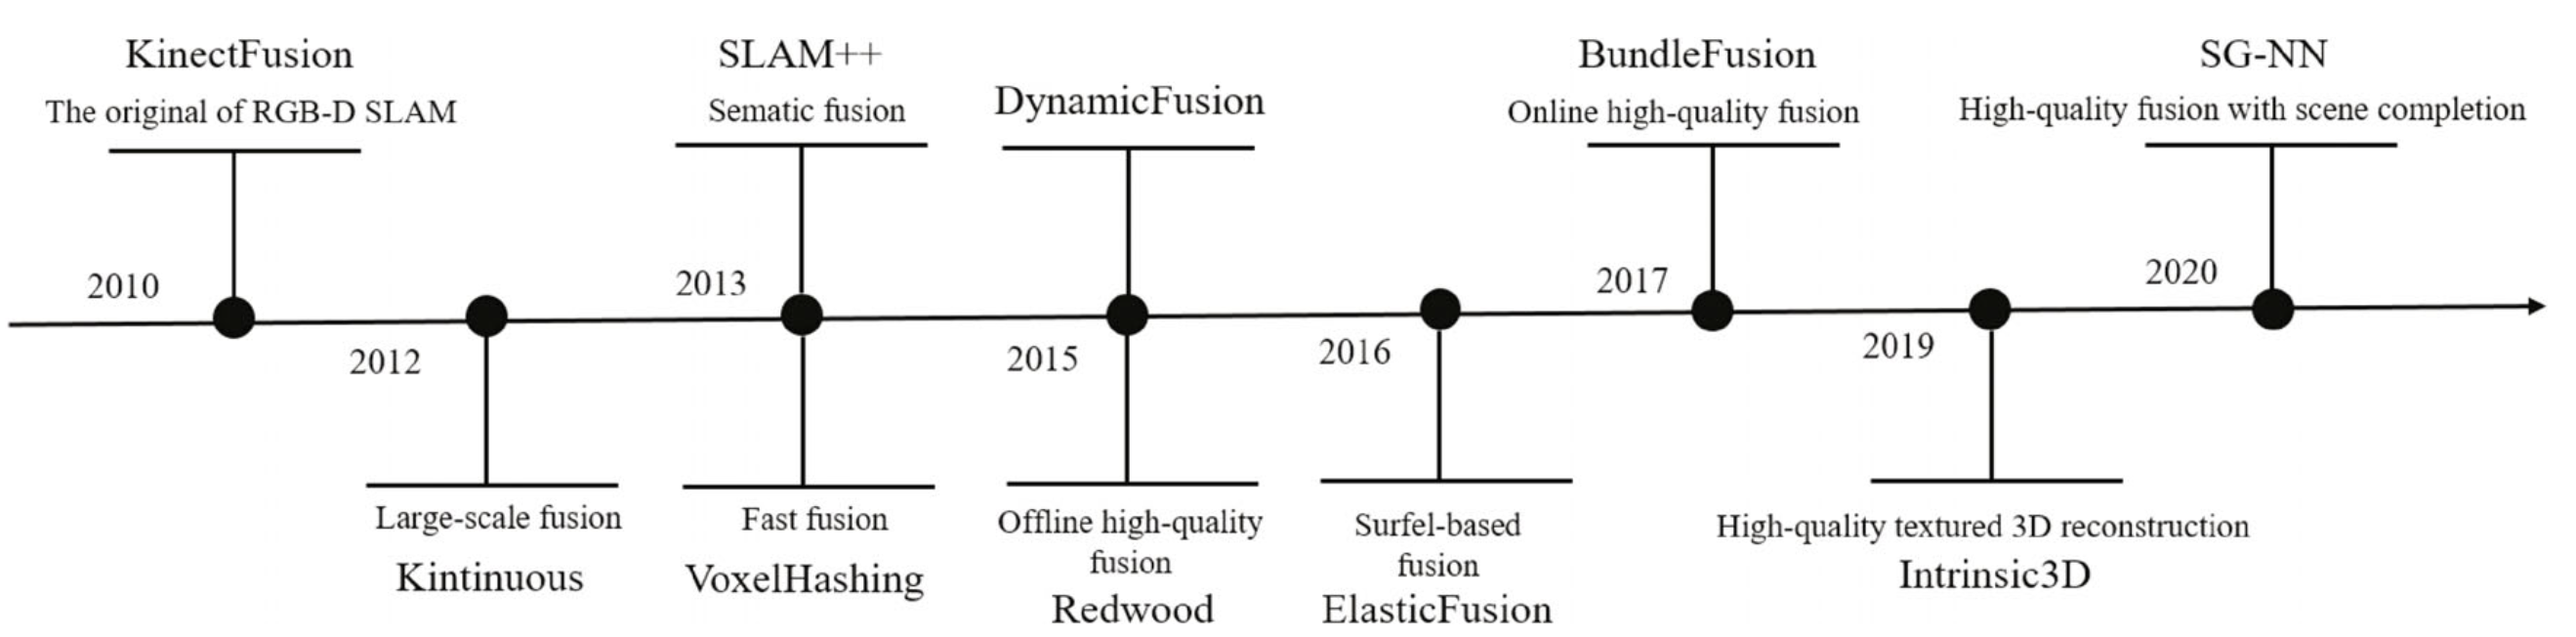
\includegraphics[width=\columnwidth]{../images/timeline of research}
	\caption{Timeline of research into 3D scene reconstruction since the influential KinectFusion paper\cite{izadi2011kinectfusion}.
	Figure from\cite{Li:2022aa}}
	\label{fig:timeline}
\end{figure}
Despite a dense body of research surrounding the topic, 3D scene reconstruction - the process of creating a 3D model of a
space from 2D data - remains an unsolved task within the field of Computer Vision, with modern systems struggling with
scenes containing dynamic (i.e.\ moving) subjects.
Figure~\ref{fig:timeline} demonstrates accelerated research efforts as a result of recent advances in RGB-D sensor technology,
stemming from the 2010 release of the Microsoft Kinect (a technology licensed from PrimeSense\cite{zhang2012microsoft}).
Since then, various other systems have been showcased, from dedicated sensors like the Asus Xtion Live, Microsoft Kinect
v2, Intel RealSense, and Azure Kinect, to integrated sensors such as those seen in Apple's iPhones and iPads (the result
of a \$345 million acquisition of PrimeSense\cite{appleprimesense}), and Tesla's self-driving cars.
\\[1ex]
Accessible consumer grade sensors facilitate and promote subject research.
One of the most notable papers in this space is KinectFusion\cite{izadi2011kinectfusion}, published in the wake of Kinect's
release.
KinectFusion proposes a system capable of dense online 3D scene reconstruction from a handheld Kinect.
Kintinuous\cite{kintinuous} and ElasticFusion\cite{elasticfusion} build on the work of KinectFusion to develop systems
which can capture scenes of a larger scale (Kintinuous), and handle more complex camera pose trajectories (ElasticFusion).
The results from these systems (and further works shown above in figure~\ref{fig:timeline}) are very compelling, but share a
common shortcoming: they struggle with dynamic scenes.

\subsection{Problem Description}\label{subsec:problem-description}
\begin{figure}[h]
	\centering
	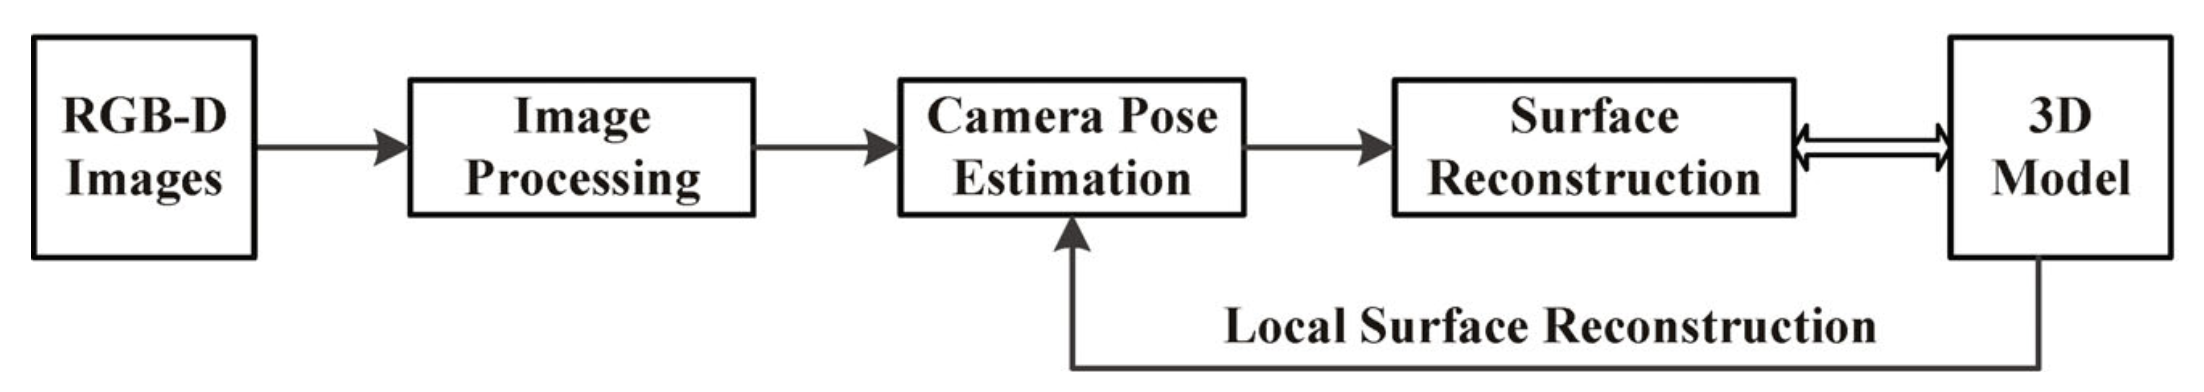
\includegraphics[width=\columnwidth]{../images/pipeline}
	\caption{Typical pipeline for 3D scene reconstruction tasks, from\cite{Li:2022aa}}\label{fig:pipeline}
\end{figure}
A standard pipeline for 3D scene reconstruction is shown in figure~\ref{fig:pipeline}.
Dynamic scenes challenge both the camera pose estimation and surface reconstruction stages of this pipeline\cite{Zhang:2018aa,berdnikov2011real}.
\\[1ex]
Camera pose estimation typically relies on Iterative Closest Point (ICP), as in\cite{kinectfusionms, elasticfusion},
which struggles to differentiate motion of moving objects from motion as a result of a moving camera.
A Sigmoid-based Iterative Closest Point (S-ICP) method is proposed by MixedFusion\cite{Zhang:2018aa}, which is quite
successful at overcoming this challenge, but the overall system fails to produce scenes with colour.
\\[1ex]
Surface reconstruction is affected by camera pose estimation (the former depends on the latter in figure~\ref{fig:pipeline}),
but another difficulty for surface reconstruction is occlusions - a surface cannot be reconstructed if depth data is not
available for it.
Berdnikov and Vatolin presented a system\cite{berdnikov2011real} which attempts to ``fill in'' holes in a depth map, but
is limited in its use by being unable to handle camera motion.
\\[1ex]
The result of these shortcomings is that current systems are unable to reliably produce artefact-free 3D reconstructions
of dynamic scenes.
This is a problem because dynamic scenes are far more commonplace than static ones\footnote{unfortunately, this trend is
not reflected in a large portion of available synthetic datasets}, therefore hindering the ability to reconstruct a majority
of scenes available in the world, e.g.\ museums, office spaces, restaurants, airports, and other high traffic public
spaces, where it is impractical to suspend public access to yield a static scene for reconstruction.

\subsection{Related Work}\label{subsec:related-work}
Some systems which work perform well in static scenes have already been discussed\cite{kinectfusionms, kintinuous, elasticfusion},
but research into systems that can reconstruct dynamic scenes is not entirely novel.
\\[1ex]
One of the earliest works in this space\cite{Keller:2013aa} proposes an online system which builds on KinectFusion\cite{kinectfusionms}.
The system leverages Izadi et al's\cite{izadi2011kinectfusion} observation - that an inability to find correspondences
between model input points during ICP suggests a dynamic object in the sampled point cloud - to segment dynamic objects
and remove them from a global point model.
\\[1ex]
DynamicFusion\cite{dynamicfusion} also builds on KinectFusion\cite{kinectfusionms}, and presents an online SLAM system
which can reconstruct non-rigidly deforming scenes.
It aims to capture a canonical\footnote{that is, ``un-warped''} version of the scene at each frame.
This allows ``traditional'' KinectFusion reconstruction to be applied, before transforming the canonical scene back into
the perceived scene.
DynamicFusion's results are \emph{very} compelling, but the system is geared towards subject capture instead of larger
scale scene capture, suffering the same limitation of KinectFusion~\cite{kinectfusionms} which Kintinuous\cite{kintinuous}
sought to address: that is, the yielded scenes are quite small.
\\[1ex]
MixedFusion\cite{Zhang:2018aa} proposes a novel S-ICP method which decouples camera motion from dynamic object motion,
facilitating more reliable camera pose estimation.
MixedFusion also contributes a key observation - some dynamic subjects can be safely removed from the scene (humans,
animals) but there are other dynamic objects which \emph{are} a part of the scene, for example: curtains, doors, tables,
chairs.
Zhang et al.\ therefore distinguish between dynamic objects with ``small'' motions which need to be preserved in the scene
and those which have more significant motion and do not constitute part of the scene.

\subsection{Project Aim}\label{subsec:proposed-project}
To address deficiency in available systems, this paper proposes a project that will build on existing systems to better
handle indoor scenes containing dynamic subjects.
\subsubsection{Objectives}
\begin{itemize}
	\item explore existing systems which operate on \emph{static} scenes;
	\item review methods for detection of dynamic objects within a scene;
	\item implement algorithms to identify dynamic objects to enable reliable camera pose estimation for the static part
	of a dynamic scene;
	\item evaluate resultant system's ability to reconstruct a crowded indoor scene;
	\item identify scope for future works.
\end{itemize}

\subsection{Project Applications}\label{subsec:project-applications}
Dynamic 3D scene reconstruction presents some exciting new applications, for example: video conferencing in VR~\cite{Campbell2019UsesOV};
Simultaneous Localisation and Mapping (SLAM) for robotics and autonomous vehicles;
virtual property viewings~\cite{virtualviewing};
preservation of culturally significant locations;
video game map generation.
The wide range of domains that this research impacts is a strong indicator of its importance.
